\RequirePackage [orthodox] {nag}

\documentclass [twoside,a4paper,11pt,french] {report}
    
    % Règles de typographie françaises
    \usepackage[french]{babel}

    % Jeu de caractères UTF-8
    \usepackage[utf8]{inputenc}
    \usepackage[T1]{fontenc}

    \usepackage {color}

    % Inclure la bibliographie dans la table des matières comme une section
    \usepackage [numbib] {tocbibind}	% numbib : section numérotée

    \usepackage{algpseudocode}

    % Fonte élégante
    \usepackage{mathpazo}
    \usepackage [scaled] {helvet}
    \usepackage{courier}

    % pour \EUR
    \usepackage{marvosym}

    % \usepackage{emptypage}

    % Utilisation de tableaux
    \usepackage{tabularx}

    % Utilisation d'url
    \usepackage{hyperref}
    \urlstyle{sf}

    % Utilisation d'images
    \usepackage{graphicx}
    \setkeys{Gin} {keepaspectratio}	% par défaut : conserver les proportions

    % Définition des marges
    \usepackage [margin=25mm, foot=15mm] {geometry}

    \parskip=2mm
    \parindent=0mm

    \pagestyle{plain}

\begin{document}

%%%%%%%%%%%%%%%%%%%%%%%%%%%%%%%%%%%%%%%%%%%%%%%%%%%%%%%%%%%%%%%%%%%%%%%%%%%%%%
% Page de garde
%%%%%%%%%%%%%%%%%%%%%%%%%%%%%%%%%%%%%%%%%%%%%%%%%%%%%%%%%%%%%%%%%%%%%%%%%%%%%%

\begin{center}
    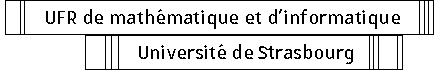
\includegraphics [width=8cm] {logo-ufr.pdf}       

    \vfill

    {
	\large
	\textsc{
	    Master d'informatique \\
	    Parcours I3D - IIRVIJ \\
		Imagerie 3D - Informatique Image Réalité Virtuelle Interaction et Jeux
	}
    }

    \bigskip\bigskip
    \bigskip\bigskip

    {\huge Rapport de projet}

    \bigskip\bigskip

    % Identité de l'auteur
    {\large Pierre \textsc{EVEN}}

    % Contact mail ou téléphone   
    {\small pierre.even@etu.unistra.fr}

    
    \vfill

    % Titre du TER : mettez un titre utile
    {
	\huge
	\textsc{
		Implémentation du jeu \\
	    ~ \\
        Pacman de 1980 en C++.
	}
    }

    \vfill
    \vfill

    \today

    \vfill

    {\large Projet réalisé avec}

    \medskip

    {
		\large Thomas \textsc{Torterotot} \small{thomas.torterotot@etu.unistra.fr}
	}

    \bigskip

    \bigskip
\end{center}

%%%%%%%%%%%%%%%%%%%%%%%%%%%%%%%%%%%%%%%%%%%%%%%%%%%%%%%%%%%%%%%%%%%%%%%%%%%%%%
% Table des matières
%%%%%%%%%%%%%%%%%%%%%%%%%%%%%%%%%%%%%%%%%%%%%%%%%%%%%%%%%%%%%%%%%%%%%%%%%%%%%%

{
    \parskip=0pt
    \tableofcontents
}
\begin{center}
    Historiquement, le jeu avait pour nom initial "PuckMan", nom qui sera par la suite changé \\
    en PacMan suite au passage de petits rigolos en ayant profité pour faire\\
    une mauvaise blague bien évidente.
    ~ \\
    Notre projet reprends ce noms original en hommage.
\end{center}

% Page blanche entre la table des matières et le texte
\cleardoublepage

%%%%%%%%%%%%%%%%%%%%%%%%%%%%%%%%%%%%%%%%%%%%%%%%%%%%%%%%%%%%%%%%%%%%%%%%%%%%%%
% Chapitre 1
%%%%%%%%%%%%%%%%%%%%%%%%%%%%%%%%%%%%%%%%%%%%%%%%%%%%%%%%%%%%%%%%%%%%%%%%%%%%%%

\chapter{Travail réalisé}
    Le programme rendu reproduit plus ou moins fidèlement le comportement du jeu Pacman de 1980.
    Il est à noter que cette fidélité est suggestive, voici un résumé des fonctionnalités et
    différences avec le jeu original :
    \begin{itemize}
        \item Seul le gameplay principal a été reproduit, les menu et cinématiques ont été ignorés. 
        (par manque de temps, et le moteur n'est pas assez développé pour permettre l'implémentation
        rapide de ce genre de fonctionnalités)
        \item La gestion des coordonnées est gérée en interne sur des doubles, ce qui peut valoir des petits 
        écarts de comportement avec le jeu initial. Ce choix permet néanmoins un rendu plus fluide et est plus
        adapté aux plétores de taux de rafraichissement différents que l'ont peut trouver sur un écran moderne.
        \item Les sprites et la map ne sont pas exactement ceux du jeu original (Ils correspondent à la version NES).
        Nous nous en sommes rendu compte tardivement ce qui nous a empéché de les corriger. 
        Nous l'avons tout de même modifiée pour être plus pratique à utiliser.
        \item Aucun systeme de rendu de texte n'a encore été implémenté dans le moteur, c'est pourquoi il n'y a aucun
        text visible dans le jeu. (les scores sont tout de même gérés et visibles dans la console)
        \item Manger une pac-gomme ou un fantôme ne ralentit / freeze pas le jeu contrairement au jeu original.
        Je trouve personnellement que c'est mieux comme ça car ça rend le jeu plus fluide.
        \item Le redimensionnement de la fenêtre est "en théorie" traité, mais il doit manquer quelques petits
        ajustements pour qu'il fonctionne sans bugs. C'est pourquoi il n'est pas disponible dans le programme fourni.
        (c'est un cas qui n'avait pas été prévu dans la conception initiale)
        \item Certains bugs du jeu original sont resimulés (ex sur l'IA des fantômes)
        \item L'algorithme de déplacement du joueur est le même que celui des fantomes, contrairement au jeu initial
        où le joueur est autorisé à "couper" les virages.
        \item Les fantômes ne sont pas ralentis dans le tunnel.
    \end{itemize}

    Pour le reste, tout suit plus ou moins fidèlement les algorithmes et comportements du jeu initial.
    (scores, vitesses, niveaux...)

\chapter{Implémentation et fonctionnement}
    Le programme est séparé en deux parties : le moteur et le jeu. Le moteur contient toute la partie utilitaire,
    rendu graphique et gestions de sprites. Celui-ci est conçu pour être
    réutilisable dans le contexte d'un autre jeu 2D utilisant des sprites simples. \\
    La partie jeu contient toutes les classes spécifiques au jeu PacMan.

\section{Le moteur}

\section{Le jeu}
\chapter{Limites et problèmes connus}
    bugs connus : Fantomes décalés / fantomes bloqués au spawn / fruit raté des fois ?
    // todo systeme de texte et 
\end{document}
